\newpage

\section{Solution}

We have implemented this problem in \emph{C++} language as a \emph{graphical user interface} application. User can choose the \emph{chessboard size} and the \emph{initial position} of knight on the chessboard. Then he can choose \emph{searching for a solution} and if a solution has been found, the application shows the solution and if solution does not exist, the application will show the appropriate message. User can stop the searching for a solution anytime, for example when it takes too long. In Figure~\ref{fig:screenshot} there is a screenshot from the start of the application.

\begin{figure}[H]
\centering
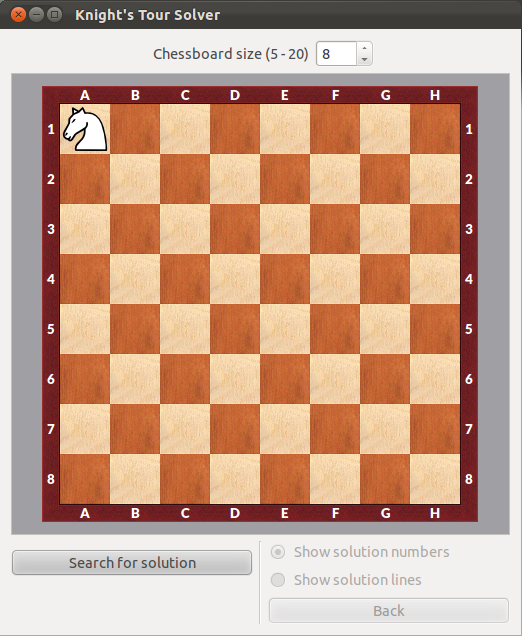
\includegraphics[width=0.8\textwidth]{screenshot.png}
\caption[Screenshot of the application]{Screenshot of the application}
\label{fig:screenshot}
\end{figure}